%%%%%%%%%%%%%%%%%%%%%%%%%%%%%%%%%%%%%%%%%%%%%%%%%%%%%%%%%%%%%%%%%%%%%%%%%%%%%
%
% Bayesian prediction of luminosity distribution based on one simulation run:
% An example from TARDIS
%
%%%%%%%%%%%%%%%%%%%%%%%%%%%%%%%%%%%%%%%%%%%%%%%%%%%%%%%%%%%%%%%%%%%%%%%%%%%%%
\documentclass[11pt]{article}
\usepackage[utf8]{inputenc}

\usepackage[a4paper, left=20mm, right=20mm, top=25mm, bottom=25mm]{geometry}
\usepackage[numbers]{natbib}
\usepackage{hyperref}
\synctex=1

\usepackage[colorinlistoftodos]{todonotes} % Use 'disable' to remove todos in final version
\newcommand{\fred}[1]{\todo[color=orange!40,inline]{#1}} %
\newcommand{\checked}{\todo[color=green,noline]{\checkmark}} %
\newcommand{\checkedl}{\todo[color=brown]{\checkmark}} %
\newcommand{\hans}[1]{\todo[color=yellow!30,inline]{#1}} %
\newcommand{\hanslong}[2][]{\todo[%bordercolor=red,
  color=white,inline,caption={2do}, #1]{
    \begin{minipage}{\textwidth} #2\end{minipage}}} %

%% CHANGE THIS DATE AS YOU MODIFY THE FILE
\newcommand{\vdate}{160309}
\pagestyle{myheadings}
\markboth{Version \vdate} {Version \vdate}
\parindent=0mm
\def\pp{\hfill\par \vspace{\baselineskip}}
%% \def\pp{}
%%%%%%%%%%%%%%%%%%%%%%%%%%%%%%%%%%%%%%%%%%%%%%%%%%%%%%%%%%%%%%%%%%%%%%%%%%%%%
\usepackage{bm,amssymb,amsfonts,amsmath}  % bold math symbols, AMStex
\usepackage{graphicx}    % standard graphics
%%%%%%%%%%%%%%%%%%%%%%%%%%%%%%%%%%%%%%%%%%%%%%%%%%%%%%%%%%%%%%%%%%%%%%%%%%%%%
\newcommand{\lleq}[1]{\label{#1} }
% TO REMOVE THE LABEL LETTERS FROM THE EQUATION DISPLAY, COMMENT OUT THIS LINE:
\renewcommand{\lleq}[1]{\label{#1} {\scriptstyle {\rm (#1)}} \hspace*{2ex} }
% \renewcommand{\labelenumi}{\arabic{section}.\arabic{subsection}.\arabic{enumi}}
% \renewcommand{\thesubsubsection}{\arabic{subsubsection}}

\newcounter{mnumi}
\newenvironment{mnumerate}{
  \begin{list}{\arabic{mnumi}.}
    {\usecounter{mnumi} \setlength{\itemsep}{0pt}
      \setlength{\leftmargin}{3ex}
    }
  }
  {\end{list}}

\newenvironment{mtemize}{
  \begin{list}{$\bullet$}
    {\setlength{\itemsep}{0pt}
     \setlength{\leftmargin}{3ex}
    }
  }
  {\end{list}}

\newcommand{\hmod}  {{\mathcal{H}}}  % Model
\newcommand{\ldef}{\;{:}{=}\;}
\newcommand{\rdef}{\;{=}{:}\;}
\newcommand{\realnumbers}{\mathbb{R}}
\newcommand{\integers}{\mathbb{Z}}
\newcommand{\cond}{\,|\,}
\newcommand{\NBD}{\mathrm{NB}}
\newcommand{\var}{\mathrm{var}}

\newcommand{\smA}{{\scriptscriptstyle A}}
\newcommand{\smB}{{\scriptscriptstyle B}}
\newcommand{\smH}{{\scriptscriptstyle H}}
\newcommand{\smK}{{\scriptscriptstyle K}}
\newcommand{\smL}{{\scriptscriptstyle L}}
\newcommand{\smM}{{\scriptscriptstyle M}}
\newcommand{\smN}{{\scriptscriptstyle N}}
\newcommand{\smR}{{\scriptscriptstyle R}}

\newcommand{\smo}{{\scriptscriptstyle 1}}
\newcommand{\smt}{{\scriptscriptstyle 2}}
\newcommand{\smr}{{\scriptscriptstyle 3}}
\newcommand{\smf}{{\scriptscriptstyle 4}}
\newcommand{\smv}{{\scriptscriptstyle 5}}
\newcommand{\smx}{{\scriptscriptstyle 6}}
\newcommand{\sms}{{\scriptscriptstyle 7}}
\newcommand{\sme}{{\scriptscriptstyle 8}}
\newcommand{\smn}{{\scriptscriptstyle 9}}

\newcommand{\bma}{{\bm{a}}}
\newcommand{\bmb}{{\bm{b}}}
\newcommand{\bmc}{{\bm{c}}}
\newcommand{\bmd}{{\bm{d}}}
\newcommand{\bme}{{\bm{e}}}
\newcommand{\bmf}{{\bm{f}}}
\newcommand{\bmg}{{\bm{g}}}
\newcommand{\bmh}{{\bm{h}}}
\newcommand{\bmi}{{\bm{i}}}
\newcommand{\bmj}{{\bm{j}}}
\newcommand{\bmk}{{\bm{k}}}
\newcommand{\bml}{{\bm{\ell}}}
\newcommand{\bmm}{{\bm{m}}}
\newcommand{\bmn}{{\bm{n}}}
\newcommand{\bmo}{{\bm{o}}}
\newcommand{\bmp}{{\bm{p}}}
\newcommand{\bmq}{{\bm{q}}}
\newcommand{\bmr}{{\bm{r}}}
\newcommand{\bms}{{\bm{s}}}
\newcommand{\bmt}{{\bm{t}}}
\newcommand{\bmu}{{\bm{u}}}
\newcommand{\bmv}{{\bm{v}}}
\newcommand{\bmw}{{\bm{w}}}
\newcommand{\bmx}{{{\bm{x}}}}
\newcommand{\bmy}{{\bm{y}}}
\newcommand{\bmz}{{\bm{z}}}
\newcommand{\bmA}{{\bm{A}}}
\newcommand{\bmB}{{\bm{B}}}
\newcommand{\bmC}{{\bm{C}}}
\newcommand{\bmD}{{\bm{D}}}
\newcommand{\bmE}{{\bm{E}}}
\newcommand{\bmF}{{\bm{F}}}
\newcommand{\bmG}{{\bm{G}}}
\newcommand{\bmH}{{\bm{H}}}
\newcommand{\bmI}{{\bm{I}}}
\newcommand{\bmJ}{{\bm{J}}}
\newcommand{\bmK}{{\bm{K}}}
\newcommand{\bmL}{{\bm{L}}}
\newcommand{\bmM}{{\bm{M}}}
\newcommand{\bmN}{{\bm{N}}}
\newcommand{\bmO}{{\bm{O}}}
\newcommand{\bmP}{{\bm{P}}}
\newcommand{\bmQ}{{\bm{Q}}}
\newcommand{\bmR}{{\bm{R}}}
\newcommand{\bmS}{{\bm{S}}}
\newcommand{\bmT}{{\bm{T}}}
\newcommand{\bmU}{{\bm{U}}}
\newcommand{\bmV}{{\bm{V}}}
\newcommand{\bmW}{{\bm{W}}}
\newcommand{\bmX}{{\bm{X}}}
\newcommand{\bmY}{{\bm{Y}}}
\newcommand{\bmZ}{{\bm{Z}}}

\newcommand{\bmalpha}{{\bm{\alpha}}}
\newcommand{\bmbeta}{{\bm{\beta}}}
\newcommand{\bmchi}{{\bm{\chi}}}
\newcommand{\bmdelta}{{\bm{\delta}}}
\newcommand{\bmepsilon}{{\bm{\varepsilon}}}
\newcommand{\bmphi}{{\bm{\phi}}}
\newcommand{\bmgamma}{{\bm{\gamma}}}
\newcommand{\bmeta}{{\bm{\eta}}}
\newcommand{\bmiota}{{\bm{\iota}}}
\newcommand{\bmkappa}{{\bm{\kappa}}}
\newcommand{\bmlambda}{{\bm{\lambda}}}
\newcommand{\bmmu}{{\bm{\mu}}}
\newcommand{\bmnu}{{\bm{\nu}}}
\newcommand{\bmomega}{{\bm{\omega}}}
\newcommand{\bmpi}{{\bm{\pi}}}
\newcommand{\bmpsi}{{\bm{\psi}}}
\newcommand{\bmrho}{{\bm{\rho}}}
\newcommand{\bmsigma}{{\bm{\sigma}}}
\newcommand{\bmtau}{{\bm{\tau}}}
\newcommand{\bmtheta}{{\bm{\theta}}}
\newcommand{\bmupsilon}{{\bm{\upsilon}}}
\newcommand{\bmxi}{{\bm{\xi}}}
\newcommand{\bmzeta}{{\bm{\zeta}}}

\newcommand{\refeq}[1]{Eq.~(\ref{#1})}
\newcommand{\reffig}[1]{Fig.~\ref{fig:#1}}

\DeclareMathOperator{\GammaDist}{Gamma}
\newcommand{\Kalpha}{{K_\alpha}}
\newcommand{\Kbeta}{{K_\beta}}
\newcommand{\npack}{n_p}
\newcommand{\lmax}{\ell_{\rm max}}
\newcommand{\Lmax}{L_{\rm max}}
\newcommand{\rmdx}[1]{\mbox{d} #1 \,} % differential

%%%%%%%%%%%%%%%%%%%%%%%%%%%%%%%%%%%%%%%%%%%%%%%%%%%%%%%%%%%%%%%%%%%%%%%%%%%%%
\begin{document}

\begin{center}
  \textbf{\Large Bayesian prediction of supernova luminosity  distributions}\\[8pt]
  \textbf{\Large based on simulation output: An example from TARDIS}\\[12pt]
\end{center}

\textbf{Abstract} TODO\\

\hans{Temporary addition of TOC to make it easier to find stuff. Eventually it should
disappear again.}

\tableofcontents


\newpage %
\hanslong{ %
  Hans 160228: \textbf{Summary of issues, based on v160218}. \\

  Before getting into all sorts of detail, I wanted to understand the
  major changes and developments. To my mind they are:
  \begin{enumerate}
  \item Fred discovered that the rescaling $X = L/\Lmax$ may have
    unintended advantages. TARDIS and general supernova luminosity
    spectra are highly variable because it consists not only of smooth
    blackbody spectrum, but also of strong absorption lines (emission
    also?? see 2014 MNRAS Kerzendorf, Sim et al?). Since $\Lmax$
    varies exactly like the spectrum itself, all binwise
    individual-packet distributions are rescaled to the interval
    $[0,1]$ leaving only a far weaker change of \textit{shape} of the
    distribution rather than the \textit{scale}.

  \item Just below Eq. (bsi) and also in (pmda), we had made explicit
    that we would do all the calculations for each bin separately, so
    there would be lots of fit parameters. Fred's 160218 paragraph
    starting with ``In general, the distribution \ldots'' and Eq
    (pmdb) sees significant reduction in the number of parameters if
    the above remnant dependence of $p(\bmL\cond N,\bmphi)$ in (pmda)
    on shape could be captured in a slow-varying function
    $a(\nu,\bmphi)$.

    \item Separately, Fred introduces the idea of combining elementary
    $b$-bins into compound bins with index $m$ as this improves the
    statistics.%
    \fred{This was an intermediate idea, I now removed any reference
      to it. There should be no more binning when infering $\bmphi$}

    \item The simplification for large $N$ etc permits a Gaussian
    approximation, hence Laplace, hence the key equation (pmp) may be
    simplified to some approximation, making use of the moment
    generating function eg Eq (mgd) unnecessary.%
    \fred{Yes, so you put in a lot of work to derive the equations and
      I checked them carefully but I think in the end we will not need
      them and we should then remove them from the draft}

  \item In principle, the above sounds like a very good development.
    There are some important caveats:
    \begin{enumerate}
      \item I see no detail on how to find $a(\nu,\bmphi)$. The first
      question would be if there is some numerical indication for its
      form. This seems to be equivalent to asking what the dependence
      of (say) the Gamma parameter $\alpha$ on $\nu$ is, and that is
      of course of great interest anyway.%
      \fred{Yes, that's equivalent. I just started with a polynomial
        for $a$ but that's ad-hoc.}

      \item My second comment is that $a(\nu,\bmphi)$ is probably just
      your normal parametrisation which enters best-fit algorithms.
      If we are to treat it as a best-fit parametrisation with
      metaparameters, then that may just bring back all the
      complications which we thought had disappeared. This would have
      to be investigated. If on the other hand you also want to treat
      $a(\nu,\bmphi)$ as some kind of ``constant function'', then one
      would have to set out how stable this constant function would be
      against various underlying changes. In other words, if
      calculation of $a()$ is not part of the general algorithm, how
      is it fixed? and can it be fixed for all cases?%
      \fred{I don't see what you mean by ``constant function''. The
        choice of $a$ and how it depends on $\bmphi$ is part of the
        overal model.}

      \item I think there may be a problem of combining the two
      proposed simplifications $L \to X$ and $m$ compound
      bins. Depending on the variability of the parametrisation as
      function of $\nu$, the shape of $p(\bmL\cond N,\bmphi)$ for
      single bins with large $\Lmax$ may differ significantly from the
      shape for many small bins combined into one using $m$. In other
      words, rebinning and rescaling may not be compatible.%
      \fred{No more compound bins, we just do an unbinned fit wrt
        $\bmphi$, so there is no issue}
    \end{enumerate}

  \item Once these are cleared up, we can get into the details \ldots\\

  \end{enumerate}
} %


%%%%%%%%%%%%%%%%%%%%%%%%%%%%%%%%%%%%%%%%%%%%%%%%%%%%%%%%%%%%%%%%%%%%%%%%%%%%%
\section{Introduction}

TODO: Wolfgang

%%%%%%%%%%%%%%%%%%%%%%%%%%%%%%%%%%%%%%%%%%%%%%%%%%%%%%%%%%%%%%%%%%%%%%%%%%%%%
\section{Bayesian prediction}

\textbf{HANS NOTE: I have just copied stuff in here which will be
  written up properly later.}
\begin{mtemize}
\item Generic definition of terms: data, parameter, variable
\item Define likelihood $p(x\cond\theta,\hmod)$
\item Product rule and sum rule (marginalisation)
\item Bayes' Theorem

\item Building a model $\hmod$ implies that we hypothesise both a
  likelihood $p(x\cond\bmtheta,\hmod)$ and a prior
  $p(\bmtheta\cond\hmod)$.

\item $p(D\cond\theta,\hmod)$ is the \textbf{likelihood} for $\theta$,
  given the data $D$. Note that, while the likelihood appears to be
  identical with the sampling distribution $p(D\cond\theta,\hmod)$
  both in notation and even in its functional form, these two
  quantities have a different purpose: The likelihood is a function of
  $\theta$ for fixed data $D$, while the forward probability is a
  function of $D$ for fixed $\theta$.

\item $p(\theta\cond\hmod)$ is the \textbf{prior probability} for
  $\theta$, before taking into account the information provided by the
  data $D$.

\item $p(D\cond\hmod)$ is sometimes called the \textbf{evidence}: it
  contains just the data, not any particular value of $\theta$. The
  only way to connect the ``evidence'' to the other probabilities is
  to expand it in terms of the sum rule, $p(D\cond\hmod) =
  \sum_{\theta'} p(D\cond\theta',\hmod)\;p(\theta'\cond\hmod)$. In
  this sense it can be thought of as the normalisation constant which
  ensures that the posterior is properly normalised.


\item $p(\theta\cond D,\hmod)$ is the \textbf{posterior probability}
  for $\theta$, after the data $D$ has been taken into account. Given
  a set of observations $D$, the $p(\theta\cond D,\hmod)$ gives the
  probability that $\theta$ takes on a particular value.

\item \texttt{COMMENT: the bracketed letters to the left of equations
    is a temporary aid to facilitate referencing. A change in
    definition of command} \verb=\lleq= \textbf{will make them revert
    to ordinary equation labels.}

\item \textbf{Bayes' Theorem}: In terms of these quantities, Bayes'
  theorem, the central theorem of inference is given by
  \begin{align}
    \lleq{bth}
    p(\theta\cond D,\hmod)
    &= \frac{p(D\cond\theta,\hmod)\;p(\theta\cond\hmod)}
    {p(D\cond\hmod)}
    = \frac{p(D\cond\theta,\hmod)\;p(\theta\cond\hmod)}
    {\int \rmdx{\theta'} p(D\cond\theta',\hmod)\;p(\theta'\cond\hmod)}
  \end{align}
  where the integral in the denominator is replaced by a sum if
  $\theta$ takes on discrete values.

\item Note that if the prior is uniform, it is independent of $\theta$
  and will cancel; we are then left with
  \begin{equation}
    \lleq{bthu}
    p(\theta\cond D,\hmod)
    = \frac{p(D\cond\theta,\hmod)} {\int \rmdx{\theta'} p(D\cond\theta',\hmod)}
  \end{equation}

\item \textbf{Prediction using Bayes' Theorem:} By contrast, the
  Bayesian prediction for $x_{n+1}$ makes full use of the information
  contained in previous data:
  \begin{align}
    p(x_{n+1}\cond D,\hmod)
    &= \int \rmdx{\theta'} p(x_{n+1}\cond\theta',D,\hmod)\;p(\theta'\cond
    D,\hmod)
  \end{align}
  i.e.\ all possible values of $\theta$ are taken into account. Using
  Bayes' theorem, this can be written also as
  \begin{align}
    p(x_{n+1}\cond D,\hmod)
    &= \frac{\int \rmdx{\theta'} p(x_{n+1}\cond\theta',D,\hmod)\;
      p(D\cond\theta',\hmod)\;p(\theta'\cond\hmod)}
    {\int \rmdx{\theta'} p(D\cond\theta',\hmod)\;p(\theta'\cond\hmod)}
  \end{align}
  which shows that the prediction for $x_{n+1}$ is a weighted average
  of $p(x_{n+1}\cond\theta',D,\hmod)$ with the weight given by
  \begin{align}
  \frac{p(D\cond\theta',\hmod)\;p(\theta'\cond\hmod)}
  {\int \rmdx{\theta'} p(D\cond\theta',\hmod)\;p(\theta'\cond\hmod)}
  &=
  \frac{p(D,\theta'\cond\hmod)}
  {\int \rmdx{\theta'} p(D,\theta'\cond\hmod)}
  \end{align}
\end{mtemize}

%%%%%%%%%%%%%%%%%%%%%%%%%%%%%%%%%%%%%%%%%%%%%%%%%%%%%%%%%%%%%%%%%%%%%%%%%%%%%
\section{TARDIS}

\subsection{Intro to those TARDIS aspects relevant to this paper}

TODO: Wolfgang (or in Introduction?)

\subsection{Definitions of relevant quantities}
\label{sec:dfnr}

\begin{mtemize}
\item Spectrum of luminosities in channels (or ``bins'')
  $b=0,1,\ldots,B$ is given by the telescope
\item In the simplest case, the frequency of channel $b$ is given by
  $\nu_b = \nu_0 + b\,\delta\nu$, where $\delta\nu$ is
  the bin width. In the general case, the bins are not of equal
  size. Let's then consider $\nu_b$ as the left edge of bin $b$,
  and $\nu_{B+1}$ is the right edge of the last bin; i.e., the
  maximum frequency.
  %%%
  \hans{The 2014 TARDIS paper I have seen uses wavelength $\lambda$,
    not frequency in their plots. Is Wolfgang's recent data all
    frequency data? If it is, ie if Wolfgang et al have decided to
    change to frequency, they should explain whether that will happen
    in their and our papers also. If they want to stick with
    wavelength, we should too. I think this is something Wolfgang
    should decide.

    If they say we should stay with wavelength, then I would suggest
    replacing $\nu$ by $\lambda$ here and throughout, and of course
    change the Poisson parameter below to something like $\nu$.}

  \item We treat the results of a single TARDIS run as \textit{simulated data}
    %%%%%
    \fred{If in the end we want to compare to actual data from a
      telescope, I'd prefer to not call the TARDIS output
      ``data''. Why don't we just call it ``TARDIS output''?} %
    \hans{I agree, ``data'' is awkward, and it is indeed useful to
      keep data and $D$ for later. ``Output'' would be ok, except that
      we should change the symbol $D$ to something else too. Symbol
      $O$ is not good. For the moment I would suggest $D_S$ (subscript
      simulation) or $D_T$ since we know that $T$ will later stand for
      temperature. Another useful term would be ``simdata'', symbol
      $S$.}
    %%%%%
    $S$, i.e.\ fixed results which we do not question but accept as
    given.  These ``data'' consist of the total number of packets
    leaving the supernova $\npack$ plus the set of luminosities
    $\bml$ and frequencies $\bmnu$ of each packet,
  \begin{align}
    \lleq{dfc}
    S = \{ \npack, \bml, \bmnu \} \,,
  \end{align}
  where
  \begin{align}
    \lleq{dfd}
    % \bml_b &= (\ell_{b,1},\ell_{b,2},\ldots,\ell_{b,n_b})
    \dim \bml = \dim \bmnu = \npack \,.
  \end{align}
  In terms of $\mathbf{1}_V(x)$---the indicator function requiring
  $x \in V$---the number of packets in bin $b$ is
  \begin{align}
    \lleq{dff}
    n_b = \sum_{j=1}^{\npack} \mathbf{1}_{[\nu_b,\nu_{b+1}]}( \nu_j )
  \end{align}
  and the total luminosity in bin $b$ is
  \begin{align}
    \lleq{dfe}
    \ell_b = \sum_{j=1}^{\npack}\ell_j \mathbf{1}_{[\nu_b,\nu_{b+1}]}( \nu_j )\,,
  \end{align}
  with $\npack = \sum_b n_b$ and the total supernova luminosity $\ell
  = \sum_b \ell_b$.

\end{mtemize}

\subsection{Data as realization of compound process}

While we treat the TARDIS output as fixed ``data'' as discussed above,
a repeat of the simulation with a different Monte Carlo seed would
evidently yield different ``data'' $S'$ even when all other simulation
parameters remain the same. Clearly, $n_b$ is a specific realization
of a stochastic variable $N_b$ governed by a model pdf $p(N_b)$. %
\fred{In our general case, $\npack = \sum_b n_b$ is an instance of a
  random variable because some packets leave the supernova, some
  don't. I guess in most applications the total number of events would
  be chosen and not random. We are fortunate that this difference does
  not matter because we consider bins independently. } %
\hans{I will come back to this later} %
Similarly, $\bml_b$ is a specific realization of a collection of
stochastic variables $\bmL_b =\{L_{b,1},\ldots,L_{b,\smN_b}\}$, where
the number $N_b$ of such variables is itself stochastic. The relevant
pdf for $\bmL_b$ therefore always presupposes knowledge of $N_b$, so
we must work with the conditional probability $p(\bmL_b\cond
N_b)$. This situation is captured mathematically as $N_b \sim p(N_b),
\bmL_b \sim p(\bmL_b\cond N_b)$ where $\sim$ means ``is by hypothesis
distributed in this model according to the pdf'', i.e.\
\begin{align*}
  (N_b,\bmL_b) &\ \sim\ p(N_b,\bmL_b\cond \bmphi_b,\lambda_b)
  = p(\bmL_b\cond N_b,\bmphi_b)\; p(N_b\cond \lambda_b),
\end{align*}
where $\bmphi_b$ is the set of parameters of the model pdf which
govern $\bmL_b$ and $\lambda_b$ is the parameter of the model pdf
governing $N_b$.  To simulate $(N_b,\bmL_b)$, we clearly first need to
generate one $N_b$, followed by the generation of $N$ packet
luminosities $\bmL_b$. This situation is termed a \textit{compound
  process}.

\subsection{Construction of the model hypothesis}

\begin{mtemize}
\item We omit the dependence on the physical supernova parameters
  $\bmtheta$ from the notation below and instead condition on the
  TARDIS output $\npack, \bml, \bmnu$ directly.

\item In the remainder of this paper, we assume that the packet
  multiplicities $N_b$ and total luminosities $\bmL_b$ in any given
  bin $b$ are statistically independent of those in other bins. %
  \fred{We could motivate this in the usual way as the Poisson limit
    of the Binomial. The subtlety would then the be the random total
    number of packets (leaving the supernova).} %
  \hans{The limit would be from the multinomial with $B$ bins and
    $\npack$ packtes to product of Poissonians. One could put it in,
    but in my opinion it's not necessary. $B$ is large, so the
    constraint plays no role.} %
  This means that the joint probability over all bins factorises into
  individual probabilities for each bin,
  \begin{align}
    \lleq{bsi}
    p(N_0,\bmL_0\ldots,N_b,\bmL_b,\ldots,N_\smB,\bmL_\smB
    \cond \npack, \bml, \bmnu,\bmphi,\bmlambda,\hmod)
    &= \prod_{b=0}^B p(N_b,\bmL_b\cond n_b, \bml, \bmnu,\bmphi,\bmlambda,\hmod)
    % p(N_0,\ldots,N_b,\ldots,N_\smB \cond \bmtheta,\bmphi,\hmod)
    % &= \prod_{b=0}^B p(N_b\cond \bmtheta,\bmphi,\hmod)\\
    % p(L_0,\ldots,L_b,\ldots,L_\smB \cond N_0,\ldots,N_\smB,\bmtheta,\bmphi,\hmod)
    % &= \prod_{b=0}^B p(L_b\cond N_b,\bmtheta,\bmphi,\hmod)
  \end{align}

\item Based on the assumption of bin-bin statistical independence, we
  shall henceforth drop the bin index and do all our calculations for
  an individual bin $b$ only, writing for example $L_b \to L, n_b \to
  n$ etc.  The total spectrum is then obtained by doing any given
  analysis or calculation for all bins. But note that while the
  single-bin probability $p(N_b,\bmL_b\cond n_b, \bml,
  \bmnu,\bmphi,\bmlambda,\hmod)$ depends only on the number of packets
  $n_b$ in the bin, it depends on the luminosities and frequencies of
  \emph{all} packets.
  %
  \fred{Perhaps it doesn't simplify the reading experience to omit $b$?}

\item Since we shall not be doing model comparison, we can for the
  moment drop the $\hmod$ from the probability notation.

\item The \textbf{model} which we construct consists of the above
  assumptions plus
  \begin{align*}
    \text{likelihood } &\ p(\bmL\cond N,\bmphi)\\
    \text{likelihood } &\ p(N\cond\lambda)\\
    \text{prior } &\ p(\bmphi)\\
    \text{prior } &\ p(\lambda)
  \end{align*}
  which are assumed to have the same functional form in each bin,
  while of course the parameter values will change from bin to bin.

\item We choose $N$ to follow a Poisson distribution \fred{this choice
    linked to limit of Multinomial, see above} with parameter
  $\lambda$ %
  \hans{I would change the Poisson parameter to $\nu$, see above comment.}
  \begin{align}
    \lleq{pmc}
    p(N\cond\lambda) &= \frac{e^{-\lambda}\lambda^N}{N!}
    \qquad N = 0,1,\ldots,\infty,\quad \lambda>0
  \end{align}

\item We further assume that individual packets are generated
  independently,
  \begin{align}
    \lleq{pmda}
    p(\bmL\cond N,\bmphi) &= \prod_{j=1}^N p(L_j\cond \bmphi)
  \end{align}

  \item In general, the distribution of $L_j$ could be a of a
  different functional form in each bin. For simplicity, we assume it
  is identical but may depend on parameters that differ from bin to
  bin. In practice, the distribution of packets does not change
  abruptly with frequency. We therefore assume that any parameter
  needed to fully specify $p(L_j)$ is given as a continuous function
  of frequency and parameters $\bmphi$; i.e.,
  \begin{align}
    \lleq{pmdb}
    p(L_j) = p(L_j \cond \nu, \bmphi)
  \end{align}
  For example, assume $p(L_j)$ depends on one parameter $a$. If we fit
  separately in each bin, we would have $B+1$ fits and $B+1$ copies of
  $a$. In each fit, there would be only few packets to constrain
  $a$. To avoid that, we assume $a = a(\nu, \bmphi)$. For concreteness,
  assume $\bmphi = (a_0, a_1)$ and
  \begin{align}
    \lleq{pmdc}
    a(\nu, \bmphi) = a_0 +a_1 \nu
  \end{align}
  This greatly reduces the number of parameters from $B+1$ to 2 and
  ensures that $a$ is continuous in $\nu$. $a$, or equivalently
  $\bmphi$, is now determined from a single fit to all packets. The
  uncertainty on $a$ is at a minimum for the frequency around which
  the density of packets is highest. \fred{Refer to plot with
    uncertainty band}

\item The values of $\lambda$ and $\bmphi$ are unknown. It is the task
  of the analysis below to determine not just the single best values
  for these parameters, but to take into account every and all
  possible values.

  \item Priors: metaparameter $a$
  %
  \hans{This is a placeholder to remind us that metaparameters need to
    be discussed at some point. Perhaps not here, but we should
    remember.}
\end{mtemize}

%%%%%%%%%%%%%%%%%%%%%%%%%%%%%%%%%%%%%%%%%%%%%%%%%%%%%%%%%%%%%%%%%%%%%%%%%%%%%
\section{Prediction based on individual packets}


\subsection{Predicting the packet multiplicity $N$ in a bin}

\texttt{COMMENT: The derivation below is deliberately slow; the
  intention being to give the novice an easy introduction into the
  usage of Bayes before we hit the more complicated calculations
  further below.}

We first show how to use Bayesian prediction to find the probability
distribution for $N$, the number of packets in a bin, given knowledge
of ``data'' in the form of TARDIS multiplicity $n$ for that bin.
Since $n$ is a specific
realization of $N$, it results from the same Poisson distribution
\begin{align}
  \lleq{pmcb}
   p(n\cond\lambda) &= \frac{e^{-\lambda}\lambda^n}{n!}
\end{align}
with the same value for $\lambda$ as in (\ref{pmc}).  We can hence use
Bayes' Theorem to find the posterior distribution for $\lambda$ given
data $n$ and the Poisson hypothesis
\begin{align}
  \lleq{pmd}
  p(\lambda\cond n) %
  &= \frac{p(n\cond\lambda)\,p(\lambda)} {p(n)}
  \ =\ \frac{p(n\cond\lambda)\,p(\lambda)} %
  {\int \rmdx{\lambda} p(n\cond\lambda)\,p(\lambda)}
\end{align}
to find the prediction of $N$ given $n$ taking into account all
possible values of $\lambda$,
\begin{align}
  \lleq{pme}
  p(N\cond n)
  &= \int \rmdx{\lambda}p(N,\lambda\cond n)
  \ =\ \int \rmdx{\lambda} p(N\cond\lambda, n)\,p(\lambda\cond n)
  \ =\ \frac{\int \rmdx{\lambda} p(N\cond\lambda)\,p(n\cond\lambda)\,p(\lambda)}
  {\int \rmdx{\lambda} p(n\cond\lambda)\,p(\lambda)}
\end{align}
where $p(N\cond\lambda,n) = p(N\cond\lambda)$ is independent of $n$.
Taking the prior (see Appendix)\footnote{For a uniform prior,
  the case $a{=}0$, we require of course a maximum $\lambda_{\rm
    max}$. As long as $\lambda_{\rm max}$ is large enough, the
  integral can effectively be taken to infinity.}
\begin{align}
  \lleq{pmf}
  p(\lambda) = c\lambda^{-a},
\end{align}
common choices are $a=0$ (uniform prior) and $a=1/2$ (Jeffreys
prior). Both choices lead to an improper prior but the posterior
predictive (see below) is proper.
Inserting \refeq{pmf} and (\ref{pmcb}) into (\ref{pme}), we obtain for
the evidence and the posterior predictive
\begin{align}
  \lleq{pmg}
  p(n) &= %
  \int_0^\infty d\lambda\, p(n\cond\lambda)\,p(\lambda)
  \ =\
  c \int_0^\infty d\lambda\, \frac{e^{-\lambda}\,\lambda^{n-a}}{n!}
  \ =\ c\frac{(n-a)!}{n!}
  \\
  \lleq{pmh}
  p(N\cond n) %
  &= \frac{n!}{(n-a)!} \int_0^\infty d\lambda\,
  \frac{e^{-2\lambda} \lambda^{N+n-a}}{N!\, n!}
  \ =\ \frac{(N+n-a)!}{N!\,(n-a)!\,2^{N+n+1-a}}
\end{align}
which we recognise as a Negative Binomial distribution describing the
probability to observe $N$ successes given $k=n+1-a$ failures in a
sequence of Bernoulli trials with success probability $\rho=1/2$
\begin{align}
  \lleq{pmhb}
  p(N\cond n) &= \NBD(N\cond k{=}n{+}1{-}a, \rho{=}\tfrac{1}{2})
  \ =\ \binom{N{+}n{-}a}{N}
  \left(\frac{1}{2}\right)^N \left(\frac{1}{2}\right)^{n+1-a}
\end{align}
We shall use the properties of the Negative Binomial in the
calculations below. \fred{Check if we still do later} For non-integer $a$,
the Negative Binomial generalizes immediately to the Pólya
distribution by replacing $x! \to \Gamma(x+1)$. Note that the
distribution of $N$ given $n$ is independent of $\bmL$ and $\bml$ by
construction but depends on $\bmnu$ implicitly through $n$.

\subsection{Predicting the total luminosity $L$ in a bin}

\texttt{COMMENT: We may want to eliminate some intermediate steps in
  the derivations below in the final paper. Wolfgang: how much detail
  should be supplied in the paper?}

\fred{One thing is bugging me: To predict the luminosity in a bin, I
  should do this $ \int_{\nu_b}^{\nu_{b+1}} d{\nu} \, p(L, \nu) =
  \int_{\nu_b}^{\nu_{b+1}} d{\nu} \, p(L \cond \nu) p(\nu) $. We want
  to avoid modeling $p(\nu)$ because of the absorption lines, so we
  assume $p(L \cond \nu)$ approx. indep. of $\nu$ in the bin, so $ \approx p(L \cond
  \nu ) \int_{\nu_b}^{\nu_{b+1}} d{\nu} \, p( \nu) \equiv p(L \cond
  \nu) \, p_b$. Since $p_b$ is unknown, we should marginalize over it
  using our knowledge from Tardis output:
  $$
  p(L \cond \mbox{bin } b, \npack, \bmnu, \bml) = \int \rmdx{p_b} p(L \cond \nu) \, p_b \, p(p_b \cond \npack, \bmnu, \bml)
  $$

  So how can we turn $\int \rmdx{p_b} p_b \to \sum_N$? Where does
  $\npack$ come into play? If we can answer this, then we have one
  more hidden assumption clarified in the derivation below that was
  written for a binned analysis but now we want to be unbinned wrt
  $\bmnu, \bml$.  }

\subsubsection{Direct probability}

% \fred{We should be more general: let's reserve $n$ for the number of
%   packets observed in a bin. Suppose this is $n=1$. From that, we can
%   hardly infer the luminosity distribution. Instead, we group the
%   packets in larger bins such that there are at least $m \gtrsim 300$
%   packets, and then assume the distribution doesn't change much with
%   frequency.

%   Hence we will learn $\bmphi$ from $m$ samples, and
%   $p(\bmphi\cond N,n,\bml) \to p(\bmphi\cond N,m,\bml)$ and we can
%   keep $\bml$ with the same meaning. So we replace $n \to m$ below
%   except in $p(N \cond n$)}

Our goal of predicting $L$ in bin $b$ given the TARDIS output
$(\npack,\bml, \bmnu)$ is captured in the probability $p(L\cond \nu,
\npack,\bml, \bmnu)$ with all relevant parameters integrated out using
the law of total probability.

To simplify the treatment, we assume that the frequency bins are
narrow or equivalently that $p(L \cond \nu, \npack, \bml, \bmnu)$ does
not vary within a bin. This implies that all hypothetical samples
$L_j$ in the bin follow the same distribution.  As the reference
frequency, we choose the bin center;
% and avoid integration over the bin
i.e., for each bin $b$, we set
\begin{align}
  \lleq{pmq}
  p(L\cond \nu, \npack,\bml, \bmnu) = p(L\cond (\nu_b + \nu_{b+1}) / 2, \npack,\bml, \bmnu)  \; \forall \nu \in [\nu_b, \nu_{b+1}] \, .
\end{align}

We first note from \refeq{pmh} that $N$ does not depend on $\bml$ at
all and only indirectly depends on $\bmnu$ through $n$, the number of
packets in the bin; cf. \refeq{dff}. Furthermore, since $L$ is fully
determined by $(N,\bmL)$,
\begin{align}
  \lleq{pmjd}
  L &= \sum_{j=1}^N L_j
\end{align}
is does not depend on $(\npack,\bml,\bmnu)$, i.e.\
\begin{align}
  \lleq{pmi}
  p(L\cond N,\nu,\bmL,\npack,\bml, \bmnu)
  = p(L\cond N, \bmL)
  &= \delta(L - \textstyle\sum_{j=1}^N L_j),
\end{align}
where the $L_j$ are assumed to occur at $\nu$.
% For notational simplicity, we now
% suppress $\nu$ and remember that all probabilities below are
% conditional on $\nu$.
Then the prediction is given by
\begin{align}
  \lleq{pmj}
  p(L\cond \nu, \npack,\bml, \bmnu)
  &= \sum_{N=0}^\infty p(L\cond N,\nu, \npack,\bml, \bmnu)\,p(N\cond \nu, \npack,\bml, \bmnu) \\
  \lleq{pmjb}
  &= \sum_N p(N\cond n)\,\int \rmdx{\bmL} p(L\cond N,\bmL,\nu, \npack,\bml, \bmnu)\, p(\bmL\cond N,\nu, \npack,\bml, \bmnu)
  \\
  \lleq{pmjc}
  &= \sum_N p(N\cond n)\,\int \rmdx{\bmL} \delta(L - \textstyle\sum_{j=1}^N L_j)
  \, p(\bmL\cond N,\nu, \npack,\bml, \bmnu)
\end{align}
The dependence on the TARDIS output $(\npack,\bml, \bmnu)$ enters
through $p(\bmL\cond N,\npack,\bml, \bmnu)$ in terms of the parameters
$\bmphi$ of $p(\bmL\cond N,\bmphi)$,
\begin{align}
  \lleq{pmk}
  p(\bmL\cond N,\nu, \npack,\bml, \bmnu)
  &= \int \rmdx{\bmphi} p(\bmL\cond N,\bmphi,\nu, \npack,\bml, \bmnu)\,p(\bmphi\cond N,\nu, \npack,\bml, \bmnu) \\
  &= \int \rmdx{\bmphi} p(\bmL\cond N,\bmphi, \nu)\,p(\bmphi\cond N,\nu, \npack,\bml, \bmnu).
\end{align}
because $\bmL$ is fully determined by $N,\bmphi, \nu$ and hence independent
of $\npack,\bml, \bmnu$.
%
Again using Bayes' Theorem (\ref{bth})
\begin{align}
  \lleq{pmkb}
  p(\bmphi\cond N,\nu, \npack,\bml, \bmnu) &=
  \frac{p(\bml\cond \bmphi, N,\nu, \npack,\bmnu)\,p(\bmphi\cond N,\nu, \npack,\bmnu)} %
  {\int \rmdx{\bmphi} p(\bml\cond \bmphi,N,\nu, \npack,\bmnu)\,p(\bmphi\cond N,\nu, \npack,\bmnu)}, %
  % \ =\ \frac{p(\bml\cond N,\npack,\bmphi)\,p(\bmphi\cond N,n)} %
  % {p(\bml\cond n)} %
\end{align}
using a multiplicity- and frequency-independent prior for $\bmphi$
\begin{align}
  \lleq{pml}
  p(\bmphi\cond N,\nu, \npack,\bmnu) &= p(\bmphi),
\end{align}
and recognizing that $\bml$ is independent of $N$ and $\nu$
\begin{align}
  \lleq{pmla}
  p(\bml\cond \bmphi,N,\nu, \npack,\bmnu) = p(\bml\cond \bmphi,\npack,\bmnu)
\end{align}
we can write (\ref{pmk}) as
\begin{align}
  \lleq{pmn}
  p(\bmL\cond N,\nu, \npack,\bml, \bmnu)
  &= \int \rmdx{\bmphi} p(\bmL\cond N,\bmphi)\, %
  \frac{p(\bml\cond \bmphi, \npack, \bmnu)\,p(\bmphi)} %
  {\int \rmdx{\bmphi} p(\bml\cond \bmphi,\npack,\bmnu)\,p(\bmphi)} \\
  \lleq{pmo}
  &= \frac{1}  {p(\bml\cond \npack, \bmnu)} %
  \int \rmdx{\bmphi} p(\bmL\cond \bmphi, N)\, %
  p(\bml\cond \bmphi, \npack,\bmnu)\,p(\bmphi)
\end{align}
with $p(\bml\cond \npack, \bmnu) = \int \rmdx{\bmphi} p(\bml\cond \bmphi,
\npack,\bmnu)\,p(\bmphi)$ in the denominator.  Inserting this into
(\ref{pmjc}), we obtain the desired result:
\begin{equation}
  \lleq{pmp}
  \boxed{
  p(L\cond \nu, \npack,\bml, \bmnu)
  = \frac{1}{p(\bml\cond \npack, \bmnu)}
  \sum_N p(N\cond n)\,\int \rmdx{\bmL} \delta(L - \textstyle\sum_j L_j)
  \displaystyle\int \rmdx{\bmphi} p(\bmL\cond N,\bmphi) \, p(\bml\cond \bmphi,\npack,\bmnu)
  \, p(\bmphi)
  }
\end{equation}
with
\begin{align}
  p(\bmL\cond \bmphi, N, \nu) &= \prod_{j=1}^N p(L_j\cond \bmphi, \nu), \\
  p(\bml\cond \bmphi,\npack,\bmnu) &= \prod_{j=1}^{\npack} p(\ell_j\cond \bmphi, \nu_j)
\end{align}
and $p(\cdot \cond \bmphi, \cdot)$ is the same function in both equations.
In other words: Once we have decided on a prior $p(\bmphi)$ and a
specific pdf to model the likelihood $p(L_j\cond \bmphi)$, we have a
prediction for $L$ which takes into account all possible $N$,
$\lambda$ and $\bmphi$.

\subsubsection{Moment generating function}
\label{sec:mgff}

\texttt{COMMENT Since the TARDIS ``data'' for $L_j$ is highly
  asymmetric, the model likelihood\\ $p(L_j\cond \bmphi)$ must also
  be. Hence we have to determine if a description based on moments is
  relevant! It could be that our numbers are a very bad description of
  the posterior.}
\\

\fred{Dependence on $\nu$ is suppressed in this section}

It may be possible to calculate the prediction in Eq.~(\ref{pmp})
numerically, but it will be slow due to the multiple $d\bmL$
integral. A partial solution lies in at least finding simple
expressions for the moments and cumulants (mean, variance, skewness,
kurtosis etc) of $p(L\cond n,\ell)$. This can be accomplished by first
finding the moment generating function (mgf) (see Appendix) which in
the present case is also the Laplace transform. %
\fred{On Wikipedia, the MGF is defined as $\int_0^\infty dL\,p(L\cond
  n,\bml)\,e^{+tL}$. Then there are less minus signs to worry about} %
\hans{Yes, most books seem to use the plus sign. It makes use of
  Laplace transform harder, but I am happy to use plus.} %
For the mgf, the convolution is easily accomplished:
\begin{align}
  \lleq{mgc}
  M(t;L\cond n,\bml) &= M[t\cond p(L|n,\bml)]
  \ =\ \int_0^\infty dL\,p(L\cond n,\bml)\,e^{-tL} \\
  &= \frac{1}{p(\bml\cond n)}
  \sum_N p(N\cond n)\,\int \rmdx{L} e^{-tL} \int \rmdx{\bmL} \delta(L - \textstyle\sum_j L_j)
  \displaystyle\int \rmdx{\bmphi} p(\bmL\cond N,\bmphi) \, p(\bml\cond n,\bmphi)
  \, p(\bmphi)\\
  &= \frac{1}{p(\bml\cond n)}
  \sum_N p(N\cond n)\,\int \rmdx{\bmphi}
  \prod_{j=1}^N \left[ \int \rmdx{L_j} p(L_j\cond \bmphi)\,e^{-tL_j}\right]
   p(\bml\cond n,\bmphi) \, p(\bmphi)
\end{align}
The term in the square bracket is the moment generating function of
$p(L_j\cond \bmphi)$,
\begin{align}
  \lleq{mgcb}
  M(t; L_j\cond \bmphi) &=
  \int \rmdx{L_j} p(L_j\cond \bmphi)\,e^{-tL_j}
\end{align}
and since this is the same for all packets $L_j$, we obtain
\begin{equation}
  \lleq{mgd}
  \boxed{
  M(t;L\cond n,\bml) %
  = \frac{1}{p(\bml\cond n)}
  \sum_N p(N\cond n)\,\int \rmdx{\bmphi}
  M(t; L_j\cond \bmphi)^N
   p(\bml\cond n,\bmphi) \, p(\bmphi)
   }
 \end{equation}
 \checked{}
As shown in Appendix ***, order-$q$ moments (expectation values of
$L_j^q$) of $p(L\cond n,\bml)$ can be found by taking successive
derivatives with respect to $t$,
\begin{align}
  \lleq{mge}
  E[L^q\cond n,\bml]
  &= \left(\frac{-\partial}{\partial t}\right)^q M(t;L\cond n,\bml)\biggr|_{t=0}
  \qquad q = 1,2,3\ldots
\end{align}
from which we can find the mean, variance, skewness etc of
$p(L|n,\bml)$ without knowing its form explicitly. To do so, we need
to find successive derivatives of $\left[ M(t; L_j\cond \bmphi)
\right]^N$ appearing in (\ref{mgd}). Defining the moments of
$p(L_j\cond\bmphi)$ as
\begin{align}
  \lleq{mgf}
  \mu_q(\bmphi) &= \int \rmdx{L_j} p(L_j\cond\bmphi)\,L_j^q \qquad q = 1,2,\ldots,
\end{align}
we find
\begin{align}
  \lleq{mgg}
  \left(\frac{-\partial}{\partial t}\right) %
  M(t; L_j\cond \bmphi)^N\biggr|_{t=0}
  &= N \mu_1(\bmphi)\\
  \lleq{mgh}
  \left(\frac{-\partial}{\partial t}\right)^2 %
  M(t; L_j\cond \bmphi)^N\biggr|_{t=0}
  &= N^{\underline{2}}\mu_1^2(\bmphi) + N \mu_2(\bmphi) \\
  \lleq{mgi}
  \left(\frac{-\partial}{\partial t}\right)^3 %
  M(t; L_j\cond \bmphi)^N\biggr|_{t=0}
  &= N^{\underline{3}}\mu_1^3(\bmphi) + 3N^{\underline{2}}\mu_1(\bmphi)\mu_2(\bmphi)
  + N\mu_3(\bmphi)
\end{align}
\checked{}
where
\begin{align}
  \lleq{mgj}
  N^{\underline q} &= N(N-1)\cdots (N-q+1) = \frac{N!}{(N-q)!}
\end{align}
is the $q$th falling power of $N$. Successively inserting these and
(\ref{mgd}) into (\ref{mge}), we firstly get for the mean of $L$,
given $(n,\bml)$
\begin{align}
  \lleq{mgk}
  E[L\cond n,\bml]
  &= \frac{1}{p(\bml\cond n)}
  \sum_N p(N\cond n)\,N \int \rmdx{\bmphi} \mu_1(\bmphi) \,
  p(\bml\cond n,\bmphi) \, p(\bmphi).
\end{align}
Given that $p(N\cond n)$ is a Negative Binomial pdf, the sum is trivially
found to be
\begin{align}
  \lleq{mgl}
  \sum_N p(N\cond n)\,N &= n\frac{\tfrac{1}{2}}{1-\tfrac{1}{2}} = n
\end{align}
\fred{The first moment under NB is $\frac{\rho k}{1-\rho}$, resulting in $n-a+1$. Here and below you seem to set $a=1$ implicitly. I want to carry the $a$ along.}
so that
\begin{align}
  \lleq{mgm}
  E[L\cond n,\bml]
  &= \frac{n}{p(\bml\cond n)}
  \int \rmdx{\bmphi} \mu_1(\bmphi) \, p(\bml\cond n,\bmphi) \, p(\bmphi)
\end{align}
Since the integral is an average of $\mu_1(\bmphi)$ weighted by
$p(\bmphi\cond n, \bml)$, let us give it a name. Given a function
$f(\bmphi)$, its ``$\bmphi$-expectation value'' is defined as
\begin{align}
  \lleq{mgn}
  E_\phi[ f ] &= \int \rmdx{\bmphi} f(\bmphi) \, p(\bml\cond n,\bmphi) \, p(\bmphi)
\end{align}
in terms of which
\begin{align}
  % \lleq{mgpa}
  % p(\bml\cond n) &= E_\phi[\mu_0],\\
  %%%%%%%
  \lleq{mgo}
  E[L\cond n,\bml]
  &= n\, \frac{E_\phi[\mu_1]}{p(\bml\cond n)}
  \ =\ n\,\frac{E_\phi[\mu_1]}{E_\phi[\mu_0]}
\end{align}
\fred{$n \to n-a+1$}
On taking the second derivative and using
\begin{align}
  \lleq{mgp}
  \sum_N p(N\cond n)\,N^2
  &= \frac{n(n+1)\left(\tfrac{1}{2}\right)^2}{\left(1-\tfrac{1}{2}\right)^2}
  = n(n+1)
\end{align}
\fred{I disagree. The 2nd raw moment is $\frac{k \rho (1 + k
    \rho)}{(1-\rho)^2}$ (from Mathworld with $\rho=q,1-\rho=p, k=r$
  and manually derived from the negative binomial MGF from
  Wikipedia). With $k=n-a+1$ and $\rho=1/2$, I get $(n-a+1)(n-a+3)$}
the second moment of $p(L\cond n,\bml)$ is
\begin{align}
  \lleq{mgq}
  E[L^2\cond n,\bml]
  &= \frac{1}{p(\bml\cond n)}
  \sum_N p(N\cond n)\, \int \rmdx{\bmphi}
  \left[ N^{\underline{2}}\mu_1^2(\bmphi) + N \mu_2(\bmphi)\right]
  p(\bml\cond n,\bmphi) \, p(\bmphi) \\
  &= n^2\,\frac{E_\phi[\mu_1^2]}{E_\phi[1]}
  + n \frac{E_\phi[\mu_2]}{E_\phi[1]}
\end{align}
\fred{I have
 $$
  \frac{n-a+1}{E_\phi[1]} \left( (n-a+2)E_\phi[\mu_1^2] + E_\phi[\mu_2]\right)
$$
}
so that the variance is
\begin{align}
  \lleq{mgr}
  \var(L\cond n,\bml)
  &= n^2\, \frac{E_\phi[\mu_1^2]\,E_\phi[1] -  E_\phi[\mu_1]^2}
  {E_\phi[1]^2}
  + n\, \frac{E_\phi[\mu_2]}{E_\phi[1]}
\end{align}
It is tempting to argue that the $n^2$ term is much larger than the
$n$-order term. This depends, however, on the sizes of the respective
expectation values: no a priori assumptions can be made here.
\fred{I have the more complicated
  $$
    \var(L\cond n,\bml) = \frac{n-a+1}{E_\phi[1]^2} \left( (n-a+2)E_\phi[\mu_1^2] E_\phi[1] -(n-a+1) E_\phi[\mu_1]^2 + E_\phi[\mu_2] E_\phi[1]\right)
  $$
}

\subsection{Third-order: skewness}

TODO Hans

This may be necessary because $p(L_j\cond\bmphi)$ is highly
asymmetric, while the pdf of the sum $L$ may be less so.

\fred{I agree but what would we do if we knew the skewness? For the fit, we need to evaluate the likelihood, so we'd have to build a function my moment matching. Of course with mean and variance alone, we'd use the Gaussian. But this just reduces to the central limit theorem.}



%%%%%%%%%%%%%%%%%%%%%%%%%%%%%%%%%%%%%%%%%%%%%%%%%%%%%%%%%%%%%%%%%%%%%%%%%%%%%
\section{Modeling the TARDIS packet distribution}

TODO: All (numerics and analytics)

\begin{mtemize}
\item Find the most suitable likelihood for $p(L_j\cond \bmphi)$

\item Determine how far we can integrate analytically over the
parameters

\item How stable are the results to perturbations?

\item \texttt{COMMENT Since $p(L_j\cond \bmphi)$ is highly asymmetric,
    we have to determine if a description based on moments is
    relevant! It could be that our numbers are a very bad description
    of the posterior.}

\end{mtemize}

\fred{Yes but at least if a rather large number of events is in the
  bin, this will be good enough}

\subsection{Results for Beta distribution likelihood}

The Beta probability density function (pdf) is
\begin{align}
  \lleq{btc}
  p(x\cond a,b) &= \frac{x^{a-1}(1-x)^{b-1}}{B(a,b)} \qquad
  0 < x < 1, \quad a,b > 0.
\end{align}
where $\bmphi = (a,b)$ are the parameters and
\begin{align}
  \lleq{btd}
  B(a,b) &= \frac{\Gamma(a)\,\Gamma(b)}{\Gamma(a+b)}
\end{align}
is the beta function.
%
The form of the TARDIS single-packet distribution suggests that this
is appropriate; the strong asymmetry in the TARDIS distribution leads
us to expect most likely parameter values of $b \ll a$ so that the mode
is close to $x=1$.
%
The variable $x$ is related to packet luminosities simply by
$x = L_j/L_{\rm max}$ where $L_{\rm max}$ is the largest luminosity
in the packets i.e.\ $0 < L_j < L_{\rm max}$.
%
(Remember we are considering a single bin $b$ only, and only a single
TARDIS run.)
%
Given that we want to find the $\phi$-moments of Section \ref{sec:mgff}
in terms of TARDIS simulation ``data'', we define in this section
\begin{align}
  x_j &= \ell_j/\ell_{\rm max}
\end{align}
while $x$ without subscript is used for the generic moment
calculations. The same quantities could, of course, be used in terms
of the generic variable $x_j = L_j/L_{\rm max}$. In terms of the
original ``data'' packets, the beta distribution reads
\begin{align}
  \lleq{bte}
  p(\bml\cond \ell_{\rm max},n,a,b)
  &= \prod_{j=1}^n p(\ell_j\cond \ell_{\rm max},a,b) \\
  \lleq{btf}
  p(\ell_j\cond \ell_{\rm max},a,b)
  &= \frac{1}{\ell_{\rm max}\,B(a,b)}
  \,\left(\frac{\ell_j}{\ell_{\rm max}}\right)^{a-1}
    \left(1-\frac{\ell_j}{\ell_{\rm max}}\right)^{b-1}
  \ =\ \frac{1}{B(a,b)}
  \frac{\ell_j^{a-1}\,(\ell_{\rm max}-\ell_j)^{b-1}}
  {\ell_{\rm max}^{a+b-1}}
\end{align}
\checked{}
equivalent to the form (\ref{btc}) with $x\to x_j$.
% \begin{align}
%   p(x_j\cond a,b) &= \frac{1}{B(a,b)} x_j^{a-1} (1-x_j)^{b-1}
% \end{align}
NOTE: If $\ell_{\rm max}$ changes significantly from TARDIS run to
run, then the probability calculation may have to be changed from
$p(\bml\cond \ell_{\rm max},n,a,b)$ to\\
$p(\bml\cond \ell_{\rm max},n,a,b)\,p(\ell_{\rm max}\cond
n,a,b)$. However we are supposed to deal with ONE TARDIS run, so that
$\ell_{\rm max}$ is known and fixed.  \fred{Rather: we approximate
  $p(\ell_{\rm max} \cond n, a,b)$ by $\delta(\max \ell_{b,j})$. This
  is OK is $\sum_b n_b$ is large. For numerical stability, we want to
  ensure that $x<1$, so we take the largest $\ell_{b,j}$ and multiply
  by $1 +\varepsilon, \varepsilon = 10^{-7}$}

The moments of the beta distibution are simple,
\begin{align}
  \lleq{btg}
  \mu_q(a,b) &= \int \rmdx{x} x^q\,p(x\cond a,b)
  = \frac{(a)_q}{(a+b)_q}
  = \frac{a(a+1)\cdots(a+q-1)} {(a+b)(a+b+1)\cdots(a+b+q-1)}
  \qquad q = 0,1,2,\ldots
\end{align}
with $(a)_b$ the Pochhammer symbol.
%
\\
\fred{Formula ok but to be consistent with the notation used above, we should either use the rising factorial $a^{\overline{b}}$ here or $(a)^b$ above}

\textbf{Calculations for a uniform discrete prior}

The prior is as yet unspecified. Since there is no known conjugate
prior for the beta distribution,\fred{yes it is known. But it not
  useful because the normalization can't be calculated analytically;
  see
  http://mathoverflow.net/questions/20399/conjugate-prior-of-the-dirichlet-distribution}
we resort to a simpler prior in terms of discrete values for $a$ and
$b$ to simplify the expressions. In principle, these can be any
rational numbers, but because as stated the value of $b$ is expected
to be around 30--60, we let $a$ and $b$ be integers only, $a,b, =
1,2,3,\ldots$. \fred{I don't understand this argument} Furthermore,
since Eqs.~(\ref{mgo}) and (\ref{mgr}) always involve \textbf{ratios}
of $\phi$-expectation values, we can use a uniform improper prior,
\begin{align}
  p(a,b) &= C\qquad a,b = 1,2,\ldots,\infty
\end{align}
with $C$ the improper constant which will cancel in the ratio.
% With
% this prior, the $\phi$-expectation values become
% \begin{align}
%   E_\phi[\mu_q] &= C \sum_{a=1}^\infty \sum_{b=1}^\infty
%   \mu_q(a,b)\,\prod_j \frac{x_j^{a-1}(1-x_j)^{b-1}}{B(a,b)}
% \end{align}
We now calculate $\phi$-expectation values for this case, namely
\begin{align}
  \lleq{bthi}
  E_\phi[\mu_q(a,b)] &= \sum_{a,b}\mu_q(a,b)\,p(\bml\cond \ell_{\rm max}, n,a,b)
  \,p(a,b)
  \\
  % = C \sum_{a,b=1}^\infty \mu_q(a,b)\,p(\bml\cond \ell_{\rm max}, n,a,b)\\
  \lleq{bti}
  &= C\sum_{a,b} \frac{(a)_q}{(a+b)_q}
  \frac{1}{B(a,b)} \prod_{j=1}^n \left(x_j^{a-1}(1-x_j)^{b-1}\right)
\end{align}
\checked{}
The product can be rewritten as
\begin{align}
  \lleq{btj}
  \prod_{j=1}^n \left(x_j^{a-1}(1-x_j)^{b-1}\right)
  &= \left(\prod_j x_j\right)^{a-1}\left(\prod_j(1-x_j)\right)^{b-1}
\end{align}
\fred{This equation can be skipped}
and defining
\begin{align}
  \lleq{btk}
  y &= \prod_{j=1}^n x_j \qquad z = \prod_{j=1}^n(1-x_j)
\end{align}
\checked{}
which are data quantities independent of any model or model
parameters, we get
\begin{align}
  \lleq{btl}
  E_\phi[\mu_q(a,b)] &= C\sum_{a,b} \frac{(a)_q}{(a+b)_q}
  \frac{y^{a-1}z^{b-1}}{B(a,b)}
\end{align}
\checked{}
With the help of mathematica we find
\begin{align}
  \lleq{btm}
  E_\phi[\mu_0] &= C\sum_{a,b=1}^\infty \frac{y^{a-1}z^{b-1}}{B(a,b)}
  = \frac{C}{(1 - y - z)^2}
  \\
  E_\phi[\mu_1] &= C\sum_{a,b} \frac{a}{(a+b)}
  \frac{y^{a-1}z^{b-1}}{B(a,b)}
  \nonumber\\
  \lleq{btn}
  &= \frac{C}{(y + z)^3}
  \left[
  \frac{(y + z) [2 y^2 + (z-y)(z-1)]}
  {(1 - y - z)^2 }
   + (z-y) \ln(1 - y - z)
   \right]
%   \\
%   E_\phi[\mu_2(a,b)] &= C\sum_{a,b} \frac{a(a+1)}{(a+b)(a+b+1)}
%   \frac{(1-y)^{a-1}(1-z)^{b-1}}{B(a,b)}
%   \\
%   E_\phi[\mu_1^2(a,b)] &= C\sum_{a,b} \left(\frac{a}{a+b}\right)^2
%   \frac{(1-y)^{a-1}(1-z)^{b-1}}{B(a,b)}
 \end{align}
 \checked{}
Taking ratios, we obtain
\begin{align}
  \lleq{bto}
  \frac{E_\phi[\mu_1(a,b)]} {E_\phi[\mu_0(a,b)]}
  &= \frac{(y + z) [2 y^2 +(z- y) (1 - z)] + (z-y) (1 - y - z)^2 \ln(1 - y - z)}
  {(y + z)^3}
\end{align}
and so
\begin{align}
  \lleq{btp}
  E[L\cond n,\bml] &= n \left[
  \frac{(y + z) [2 y^2 +(z- y) (1 - z)] + (z-y) (1 - y - z)^2 \ln(1 - y - z)}
  {(y + z)^3}\right]
\end{align}
is completely determined by the data $(n,\bml)$.  Similarly
\begin{align}
  E_\phi[\mu_2] &= C\sum_{a,b} \frac{a(a+1)}{(a+b)(a+b+1)}
  \frac{y^{a-1}z^{b-1}}{B(a,b)}
  \nonumber\\
  \lleq{btq} &= \frac{-1}{(1-y-z)^2 (y+z)^5} %
  \nonumber\\
  &\times\Bigl\{ 2 \Bigl[2 y^2(z+1) + yz(z-8) - (z-2) z^2\Bigr]
  (y+z-1)^2 \ln(-y-z+1)
  \nonumber\\
  &+ (y+z) \Bigl[
    y^4 - 2 y^3 (5z+3) + y^2[(22-19 z) z+4] - 4 yz (z-4) (z-1) + 4z^2 (z-1)^2
           \Bigr] \Bigr\}
  % \nonumber\\
  % &= -(1/((y+z-1)^2 (y+z)^5)) %
  % \nonumber\\
  % &\times \Bigl\{
  %   -4 y^3 + 6 y^4 - y^5 + 12 y^2 z - 16 y^3 z + 9 y^4 z + 12 y z^2 -
  %   42 y^2 z^2 + 29 y^3 z^2 - 4 z^3 - 12 y z^3 + 23 y^2 z^3 + 8 z^4 -
  %   4 z^5 \nonumber\\
  %   &+ \ln[1 - y - z] \Bigl[
  %   -4 y^2 + 8 y^3 - 4 y^4 + 16 y z - 28 y^2 z + 16 y^3 z -
  %     4 y^4 z - 4 z^2 - 26 y z^2 + 36 y^2 z^2 - 10 y^3 z^2 + 10 z^3 +
  %     8 y z^3 - 6 y^2 z^3 - 8 z^4 + 2 y z^4 + 2 z^5
  %     \Bigr]
  %   \Bigr\}
\end{align}
and
\begin{align}
  E_\phi[\mu_1^2] &= C\sum_{a,b} \frac{a^2}{(a+b)^2}
  \frac{y^{a-1}z^{b-1}}{B(a,b)}
  \nonumber\\
  \lleq{btr} %
  &= \frac{1}{y (y - z)^3}
  \Bigl\{
  (y - z) (-y + z + 2 y \ln[y]) + y (-2 + y + z)
  (\mathrm{PolyLog}[2, 1 - y] - \mathrm{PolyLog}[2, 1 - z])
  \Bigr\}
\end{align}
These have to be combined with the above to find the variance of
Eq.~(\ref{mgr}). The hope is that the complicated mathematical
expressions simplify. Either way, the variance is also a closed
solution in terms of $n$, $y$ and $z$.

\subsection{Results for the Gamma-distribution likelihood}

The Gamma distribution  with shape parameter $\alpha$ and rate
parameter $\beta$ is defined as
\begin{align}
  \lleq{gma}
  \GammaDist(x | \alpha, \beta) = \frac{\beta^\alpha}{\Gamma(\alpha)} x^{\alpha-1} e^{-\beta x} .
\end{align}
The support of $\GammaDist(x \cond \alpha, \beta)$ is $[0, \infty]$
whereas the luminosity of real packets is bounded from above and has a
peak close to but not at the boundary. \fred{refer to plot of real
  luminosity packets in some frequency bin} In order to describe the
luminosity distribution of real packets through $\GammaDist(\alpha,
\beta)$, we have to transform the luminosities. To this end, we first
take the largest luminosity of all TARDIS packets across the entire
frequency range and increase it slightly to avoid numerical
difficulties at the end point
\begin{align}
  \lleq{gme}
  \lmax \equiv (1+\epsilon) \times \max_j \ell_j,
\end{align}
where $ \epsilon=10^{-6}$.  We assume the total number of samples
across all bins is large, hence the effect of considering $\lmax$ a
constant independent of the data is negligible. We then transform the
samples $\bml \to \bmx$ as
\begin{align}
  \lleq{gmf}
  x_j \equiv 1- \frac{\ell_j}{\lmax} > 0
\end{align}
and similarly for $L \to X$, then we infer $P(X \cond \nu,  \npack, \bmx,
\bmnu)$. Only in the end, we transform back to a probability density
in $L$ via
\begin{align}
  \lleq{gmg}
  p(L  \cond \nu,  \npack, \bml, \bmnu) = p(X  \cond \nu,  \npack, \bmx, \bmnu) \frac{1}{\lmax}
\end{align}
\hans{So far, $m$ appears only in your todo comment above. I would
  suggest a short discussion of this already in Section
  \ref{sec:dfnr}. We could then simply rewrite all equations below in
  terms of $m$ rather than $b$.} %
\fred{I removed $m$ whereever I saw it except below where I define it
  explicitly}
%
We observe good agreement between the best fit of a Gamma distribution
to TARDIS packet luminosities; an example is shown shown in
\reffig{gamma}.  While not obvious at first, a major numerical
simplification arises because of the $L \to X$
transformation. Rewriting the master equation~(\ref{pmp}) formally as
\begin{align}
  \lleq{gmh}
  p(L  \cond \nu,  \npack, \bml, \bmnu) = \sum_{N} p(N \cond \nu,  n) p(L \cond N,
\nu, \npack, \bml, \bmnu)
\end{align}
we see that the right-hand side is a mixture density. In our
application, the distribution of a single luminosity, $p(L \cond N=1,
\nu, \bml, \bmnu)$ is narrow in the sense that the standard deviation
relative to the mean is at the percent level. This implies that $p(L
\cond \nu, \npack, \bml, \bmnu)$ has one mode from each $N$ and all
modes are clearly separated. The transformation $L \to x$ effects a
strong overlap between the distributions $p(X \cond N, \nu, \npack, \bmx, \bmnu)$
with similar $N$, so $p(X \cond \nu, \npack, \bmx, \bmnu)$ can be well
approximated by a unimodal distribution; see \reffig{hedgehog}.
\fred{I'm not 100 \% sure but $p(X \cond \nu, \npack, \bmx, \bmnu)$ should still
  have $N \to \infty$ modes but they aren't visible}

\begin{figure}[ht]
  \centering
  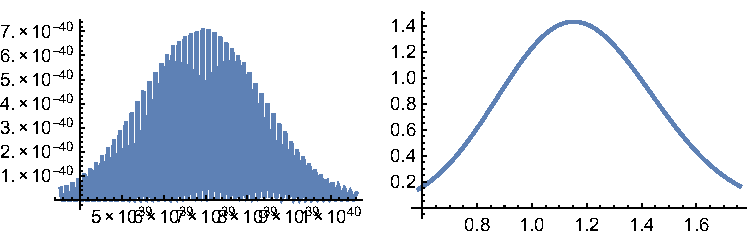
\includegraphics[width=0.48\textwidth]{hedgehog}
  \caption{Hedgehog. }
\label{fig:hedgehog}
\end{figure}


\begin{figure}[ht]
  \centering
  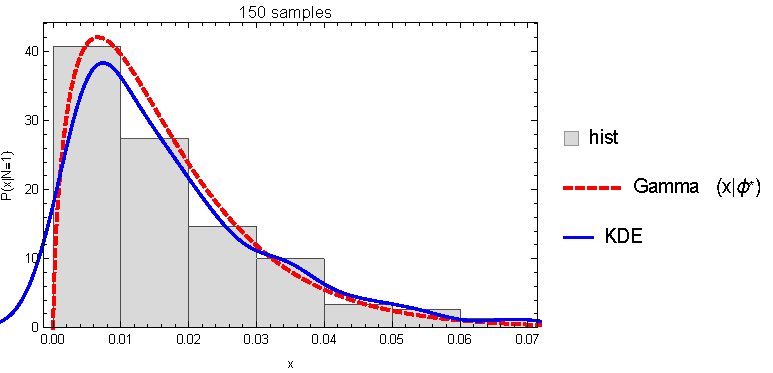
\includegraphics[width=0.48\textwidth]{gamma}
  \fred{Plot with more samples to see dip at $x=0$.} %
  \hans{I assume the KDE fit will disappear from the paper later as it
    overshoots the zero point.}
  \caption{Gamma distribution fit. }
  \label{fig:gamma}
\end{figure}

For our purposes, the most useful property of the Gamma
distribution is infinite divisibility; i.e., the sum of $N$ Gamma
variates is again a Gamma variate
\begin{align}
  \lleq{gmb}
    X_j \sim \GammaDist(\alpha, \beta) \Rightarrow X \equiv \sum_{j=1}^N X_j \sim \GammaDist(N \alpha, \beta).
\end{align}
Let us assume that $\alpha$ and $\beta$ are functions of $\nu$ with unknown parameters $\bmphi$
\begin{align}
  \lleq{gmi}
  \alpha &= \alpha(\nu \cond \bmphi),\\
  \beta &= \beta(\nu \cond \bmphi),\\
  p(X_j \cond \bmphi, \nu) &=
  \GammaDist(X_j \cond \alpha, \beta),\\
  p(\bmX \cond N, \bmphi, \nu) &= \prod_{j=1}^N p(X_j \cond \bmphi, \nu).
\end{align}
With these definitions, \refeq{gmb} is equivalent to
\begin{align}
  \lleq{gmc}
 p(X \cond N, \bmphi, \nu) &= \int \rmdx{\bmX} \delta(X - \textstyle\sum_j X_j)
  \,p(\bmX\cond N,\bmphi, \nu) = \GammaDist(X \cond N \alpha, \beta)
\end{align}
and this implies that the master equation~(\ref{pmp}) considerably simplifies as
\begin{align}
  \lleq{gmd}
    \boxed{
    p(X\cond \nu, \npack,\bmx,\bmnu)
  = \frac{1}{p(\bmx\cond \bmnu)}
  \sum_N p(N\cond n)\, \int \rmdx{\bmphi} \GammaDist(X_j \cond \alpha, \beta) % p(X \cond N, \bmphi, \nu)
  \, p(\bmx\cond \bmphi, \npack, \bmnu)
  \, p(\bmphi).
  }
\end{align}

\subsubsection*{Linear model}

In the absence of a physical model to determine $\alpha(\nu \cond
\bmphi)$ and $\beta(\nu \cond \bmphi)$, we propose to start with a simple polynomial ansatz
\begin{align}
  \lleq{gmp}
  \alpha(\nu \cond \bmphi) &= \sum_{k=0}^\Kalpha \alpha_k \nu^k,
  &\beta(\nu \cond \bmphi) &= \sum_{k=0}^\Kbeta \beta_k \nu^k
\end{align}
such that
\begin{align}
  \lleq{gmq}
  \bmphi = (\alpha_0, \dots \alpha_\Kalpha , \beta_0, \dots \beta_\Kbeta)
\end{align}
The usual trade off between parsimony and the ability to accurately
model the frequency dependence determines the orders of the
polynomials. This is outside the scope of this paper.

\subsubsection*{Priors} \label{sec:priors}

To explicitly evaluate \refeq{gmd}, we need to specify the prior
$p(\bmphi)$. To gain some insight, we first consider the special case
$\alpha = \bmphi_1$, $\beta = \bmphi_2$ where we ignore the dependence
on $\nu$; i.e., $\Kalpha = \Kbeta = 0$. For this standard $\GammaDist$
model, there is a conjugate prior but unfortunately the normalization
constant cannot be evaluated in closed form, so it is thus of no use
for us. How about a noninformative prior? The authors of
\cite{moala2013bayesian} present an overview of possible choices and
conclude that the point estimate given by the mode of the posterior is
nearly insensitive to the prior choice starting from around 30
independent identically distributed samples. We posit that there are
this many samples available near any $\nu$ under consideration, so the
prior is not crucial for our application.

There is some explicit prior information that we want to build into
our analysis. The distribution $p(x \cond \alpha, \beta)$ should
always vanish at the origin. This is equivalent to requiring a maximum
away from the boundary leading us to the condition
\begin{align}
  \lleq{gmn}
  \alpha > 1.
\end{align}

For simplicity, we choose a uniform prior on $\bmphi$ on a finite box $V$ subject to the constraint \refeq{gmn}
\begin{align}
  p(\bmphi) = \mathbf{1}_{\alpha(\bmphi) > 1}(\bmphi) \mathbf{1}_V(\bmphi).
\end{align}
The box $V$ is chosen by trial and error to be large enough to contain
the relevant region of $p(\bmx\cond \bmphi, \npack, \bmnu)$. For
simple functions $\alpha(\nu \cond \bmphi)$, one can find the minimum
value of $\alpha$ over the entire range of $\nu$ analytically. If this
is too complicated, we propose to simplify by requiring $\alpha(\nu_j
\cond \phi) > 1$ only at each packet frequency $\nu_j$. In the
evaluation of $p(\bmx \cond \bmphi, \npack, \bmnu)$, one has to loop
over all packets and compute $\alpha$ and $\beta$ anyways, so the
constraint imposes essentially no computational overhead.

\subsection{Approximations}

To explicitly evaluate \refeq{gmd}, we have to overcome the remaining
two difficulties: the sum over $N$ and the integral over
$\bmphi$. Translated to our problem, this would be 30 packets at the
\emph{same} frequency. But TARDIS only outputs packets at
\emph{different} frequencies. In the following, let $m$ denote the
effective number of packets close to $\nu$ where ``close'' is
deliberately left unspecified.  If $m$ is large, we can well determine
$\phi$ and thus $p(X_j \cond N, \bmphi, \nu)$.

% We require in addition that the posterior is narrow enough so we
% group samples in bins to have at least $m=150$ samples in each
% bin. This implicitly assumes that the luminosity distribution is
% constant in the frequency range defined by $m$.

% Note that the bins defined by the experiment in general do not overlap
% with the bins used to infer the luminosity distribution; i.e., $n \ne
% m$.

The following approximations can be used in different regions of the
parameter space spanned by $n$, $N$, and $m$. %
\hans{$n$ is TARDIS output ``data'', so not a parameter. From the
  above paragraph, $m$ seems to be a parameter governing rebinning to
  nonuniform bins. I would have no idea how to handle $m$ formally in
  a Bayesian way. If $m{=}150$ is the result of optimising the fitting
  stability, then presumably it will be kept constant. In that case,
  it would be treated like a constant rather than a parameter in the
  usual sense.}
\fred{Yes, $n$ is fixed from TARDIS output. $m$ is defined only for this paragraph}
\fred{Update approximations: don't need moments any longer}

\subsubsection*{Large $\bmn$} \label{large-n}

For large $n$, the cumulative of the Negative Binomial $p(N \cond n)$
can be approximated by the cumulative of a Gaussian with mean $n$ and
variance $2 (n - a + 1)$. Intuitively, this variance arises because the
Poisson variance appears twice, once when observing $n$ and once when
predicting $N$ given $n$.  The region around $N=n$ yields the dominant
contribution to the sum over $N$ in \refeq{gmd}. The contribution
around $N=0$ is then negligible, and we can approximate $\sum_N$ by
$\int \rmdx{N}$. The density $p(N \cond n) P(X \cond N, \npack, \bmx,
\bmnu)$ is close to a Gaussian (in the $x$ parametrization) and the
integral can be accurately approximated by Laplace's method which
requires the Hessian and the mode.
  % as each moment has to be
  % normalized by the evidence $p(\bmx \cond m)$.
The former is available in closed form and the latter has to be
determined numerically. Fortunately, Newton's method leads to a
solution in only a few steps~\cite{minka2002estimating}.
%
\fred{The reference is for max. likelihood of a $\GammaDist(\cdot)$
  but I'm sure the performance is similar for max. posterior and the
  first moments} We benefit from partial error cancelation when we
apply Laplace's method both in the numerator and
denominator~\cite{tierney_accurate_1986}.
  %
\fred{Might actually evaluate numerator and denominator at posterior
  mode to do only one instead of two optimizations;
  cf.~\cite{lindley_approximate_1980}}

\subsubsection*{Large $\bmN$} \label{large-N}

The central limit theorem states that for large $N$, $P(X \cond N,
\bmphi, \nu) \approx \mathcal{N}(X \cond N \, E_\bmphi[X_j \cond \nu],
N \, V_\bmphi[X_j \cond \nu])$. The expectation values have no known
closed-form solutions but we can easily and accurately approximate
them with Laplace's method.
% This is true independent of our model
assumption \refeq{gmi} that $X_j \sim \GammaDist(\alpha, \beta)$.
%
\fred{This only helps because the Laplace approx. when combined with
  large $n$ has an analytical result for the mode which saves us
  numerical optimization. But it requires extra (Laplace
  approximated?) integrals to compute $E_\bmphi[X_j \cond \nu]$ and
  $V_\bmphi[X_j \cond \nu]$. I can't get the Hessian analytically for
  $\npack$ samples. But we could use \texttt{Hesse} from
  \href{http://seal.web.cern.ch/seal/snapshot/work-packages/mathlibs/minuit/}{Minuit}
  or similar to approximate the Hessian at the mode by finite
  differences.}

\subsubsection*{Large $\bmm$}\label{large-m}

By asymptotic normality, the posterior $p(\bmphi \cond \npack, \bmx,
\bmnu) = p(\bmx\cond \bmphi, \npack, \bmnu) \, p(\bmphi) / p(\bmx
\cond \npack, \bmnu)$ approaches a multivariate Gaussian. In the limit
$m \to \infty$, the covariance of the posterior $p(\bmphi \cond
\npack, \bmx, \bmnu)$ tends to zero as $1/m$ and we can then fix the
parameters $\bmphi$ at the posterior mode $\bmphi^*$; i.e., $p(\bmphi
\cond \npack, \bmx, \bmnu) \to \delta(\bmphi - \bmphi^*)$ which removes the integral in \refeq{gmd}.

\subsubsection*{Large $\bmn, \bmN$,  and very large $\bmm$} \label{large-n-large-m}

With many samples observed in a narrow bin, both $n$ and $m$ are large
and the dominant contribution to \refeq{gmd} arises from large
$N$. Combining all of the above approximations, we find
\begin{align}
  \lleq{gmr} %
  p(X\cond \nu, \npack,\bmx,\bmnu) &= %
  \int \rmdx{N} \mathcal{N}(N \cond n, 2 (n -a + 1)) \, \mathcal{N}(X \cond
  N \, E_{\bmphi^*}[X_j \cond \nu], N \, V_{\bmphi^*}[X_j \cond \nu])
\end{align}
where
\begin{align}
  \lleq{gms}%
  E_{\bmphi^*}[X_j \cond \nu] &= \frac{\alpha(\nu \cond
    \bmphi^*)}{\beta(\nu \cond \bmphi^*)}, & %
  V_{\bmphi^*}[X_j \cond \nu] = \frac{\alpha(\nu \cond
    \bmphi^*)}{\beta(\nu \cond \bmphi^*)^2}.
\end{align}
Again, this integral does not have a closed-form expression but it is
unimodal and can be well approximated with Laplace's method. The mode
of the integrand is the single real root of a cubic polynomial. We
compute the root as well as the Hessian analytically with mathematica; the results are lengthy and not shown here.

\subsubsection*{Comparison of approximations}

Numerically, the most challenging case is small $n$ because the sum
over $N$ in \refeq{gmd} has to be computed explicitly starting at
$N=1$ until contributions become negligible. Since $p(N \cond n)$
falls off quickly, it is sufficient in our application to do this
until $n \lesssim 20-30$. Beyond that, we use approximations
\ref{large-n}--\ref{large-n-large-m}.

%%%%%%%%%%%%%%%%%%%%%%%%%%%%%%%%%%%%%%%%%%%%%%%%%%%%%%%%%%%%%%%%%%%%%%%%%%%%%
\section{Results}

In \reffig{beta} is a fit of the Beta distribution to 3000
samples from a TARDIS run with frequencies in the range $[1.367,
1.435] \times 10^{38}$ Hz. A characteristic feature seen in many such
similar fits is that the Beta distribution does not give a perfect
fit: it undershoots around the mode and overshoots around
$x=0.96$. The reason may be that the Beta itself is not flexible
enough to describe the data, or the distribution is simply not
constant in frequency, so we should choose smaller bins or less
samples. We don't expect 3000 samples in every bin, so what is the
minimum number of samples needed to work robustly? The first numerical
challenge is how to normalize the luminosities, I take the maximum
across all samples (not just one bin) and multiply by $10^{-6}$ to
avoid $x=1$ for any sample. For too few samples, the fit returns a pdf
that peaks at the boundary $x=1$, this is not what we want. From trial
and error, 300 samples is a solid minimum to get a robust fit if
parameters are estimated via maximum likelihood. The method-of-moment
estimator has the advantage of not requiring an optimization algorithm
but for some bins it gives a solution peaking at $x=1$ even for 800
samples so it's not robust.

\begin{figure}[ht]
  \centering
  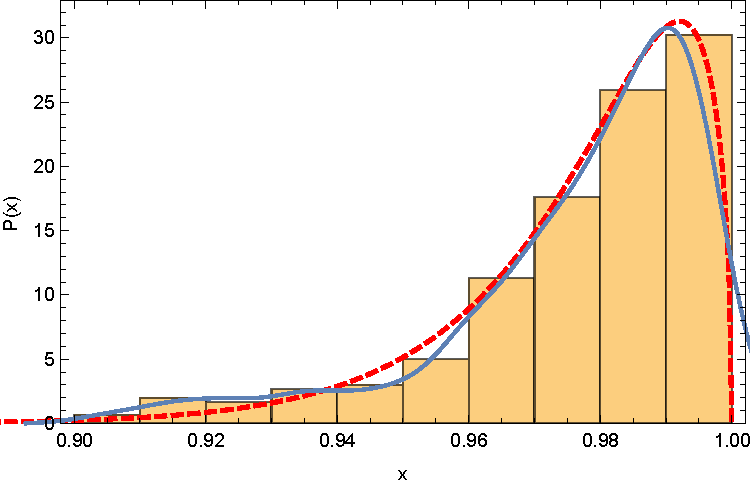
\includegraphics[width=0.48\textwidth]{beta-300}
  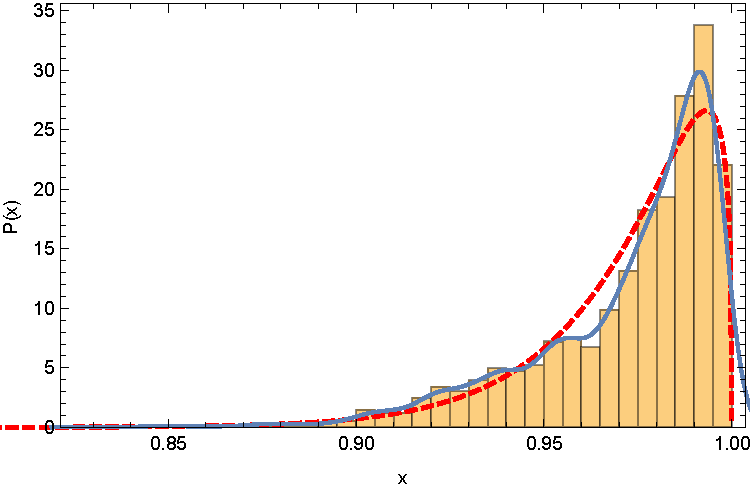
\includegraphics[width=0.48\textwidth]{beta-3000}
  \caption{Beta distribution fit. The samples are binned in the
    histogram. The blue solid curve is a kernel-density estimate, the
    red dashed curve is the Beta distribution. left: 300 samples,
    right: 3000 samples}
  \label{fig:beta}
\end{figure}

%%%%%%%%%%%%%%%%%%%%%%%%%%%%%%%%%%%%%%%%%%%%%%%%%%%%%%%%%%%%%%%%%%%%%%%%%%%%%
\section{Discussion and Conclusions}

TODO: All

%%%%%%%%%%%%%%%%%%%%%%%%%%%%%%%%%%%%%%%%%%%%%%%%%%%%%%%%%%%%%%%%%%%%%%%%%%%%%
\section*{Acknowledgements}

This work was supported in part by the DFG cluster of excellence
``Origin and Structure of the Universe'' (www.universe-cluster.de) and
the National Research Foundation of South Africa, etc etc.

%%%%%%%%%%%%%%%%%%%%%%%%%%%%%%%%%%%%%%%%%%%%%%%%%%%%%%%%%%%%%%%%%%%%%%%%%%%%%
\section{Appendix: Relevant distributions}

TODO: Hans

\subsection{Product rule and sum rule}

\subsection{Poisson}

\subsection{Negative Binomial}

%%%%%%%%%%%%%%%%%%%%%%%%%%%%%%%%%%%%%%%%%%%%%%%%%%%%%%%%%%%%%%%%%%%%%%%%%%%%%
\section{Appendix: Generating functions}

TODO: Hans
$\pi(\alpha, \beta) \propto \left( \frac{\Gamma(\alpha+\beta)}{\Gamma(\alpha) \Gamma(\beta)} \right)^{\lambda +1} (x x_0)^{\alpha-1} \left(y_0 (1-x) \right)^{\beta-1}$

%%%%%%%%%%%%%%%%%%%%%%%%%%%%%%%%%%%%%%%%%%%%%%%%%%%%%%%%%%%%%%%%%%%%%%%%%%%%%
% \section{}


%%%%%%%%%%%%%%%%%%%%%%%%%%%%%%%%%%%%%%%%%%%%%%%%%%%%%%%%%%%%%%%%%%%%%%%%%%%%%
\bibliographystyle{plain}
\bibliography{references}

%%%%%%%%%%%%%%%%%%%%%%%%%%%%%%%%%%%%%%%%%%%%%%%%%%%%%%%%%%%%%%%%%%%%%%%%%%%%%
\end{document}
%%%%%%%%%%%%%%%%%%%%%%%%%%%%%%%%%%%%%%%%%%%%%%%%%%%%%%%%%%%%%%%%%%%%%%%%%%%%%

% Local Variables:
% compile-command:"rubber --pdf -W refs -S bayes-tardis-luminosity-prediction"
% End:
